\begin{surferPage}{이중 원뿔}
   앞서 소개란에 설명되었듯이 곡면이 갖는 뾰족한 점을 \textit{특이점} 이라 부릅니다. 특이점을 갖지 않는 곡면을 \emph{비-특이} 혹은 \emph{매끄러운} 곡면이라고 부릅니다. 예를 들면 구나 도넛(아래에서 왼쪽  두 그림)은 특이점을 갖지 않습니다. 
    \begin{center}
      \vspace{-0.1cm}
      \begin{tabular}{@{}c@{}c@{}c@{}c@{}}
        \begin{tabular}{@{}c}
          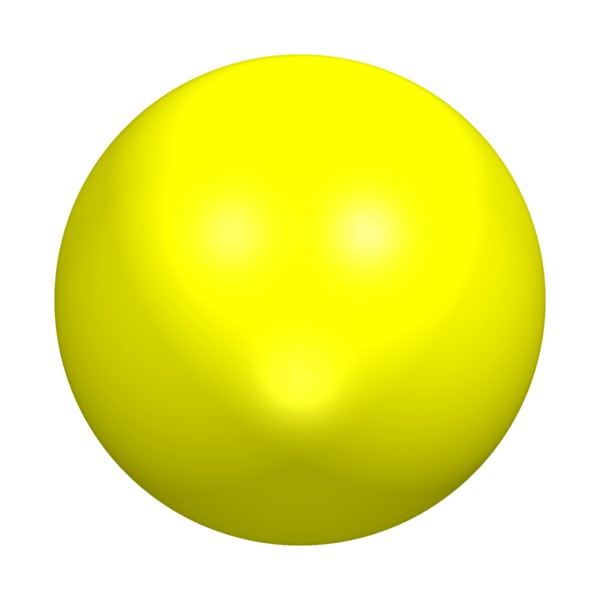
\includegraphics[width=1.4cm]{./../../common/images/kugel}
        \end{tabular}
        &
        \begin{tabular}{@{}c}
          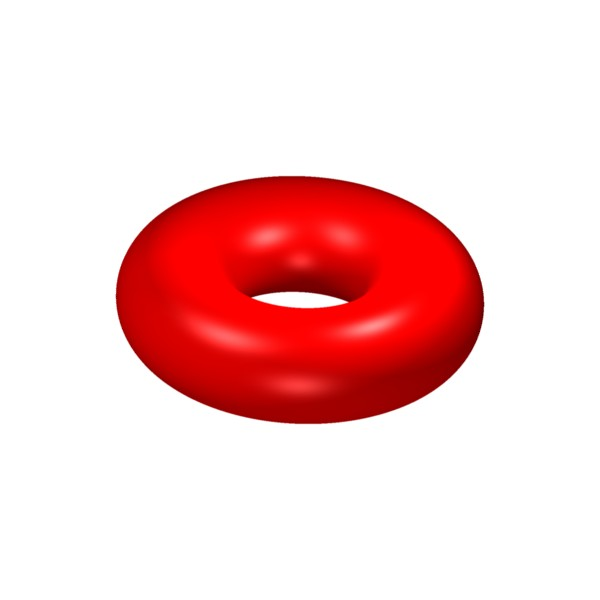
\includegraphics[width=1.4cm]{./../../common/images/torus}
        \end{tabular}
        &
        \begin{tabular}{c@{}}
          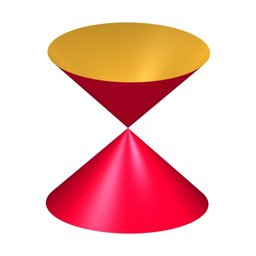
\includegraphics[width=1.4cm]{./../../common/images/kegel}
        \end{tabular}
      \end{tabular}
    \end{center}
    \vspace{-0.3cm}
    위의 맨오른쪽의 이중 원뿔은 가장 간단한 형태의 특이점을 갖습니다. $2$차 다항식으로 표현되는 유일한 특이점이기도 하지요.
    \[x^2+y^2-z^2=0.\]
    $0$ 대신 작은 변수 $a$를 넣어서 이 식을 아주 조금만 변형시키면 부호에 따라 두 가지 종류의 쌍곡면이 만들어집니다. 오른쪽 막대를 이용하여 확인해 보십시오!

%    \dontshow{
    % 
    \begin{center}
      \vspace{-0.2cm}
      \begin{tabular}{@{}c@{\ }c@{\ }c@{\ }c@{\ }c@{}}
        \begin{tabular}{@{}c@{}}
          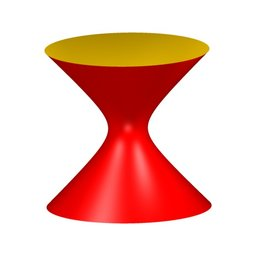
\includegraphics[width=1.2cm]{./../../common/images/A1pm_2}
        \end{tabular}
        &
        $\leftarrow$
        &
        \begin{tabular}{@{}c@{}}
          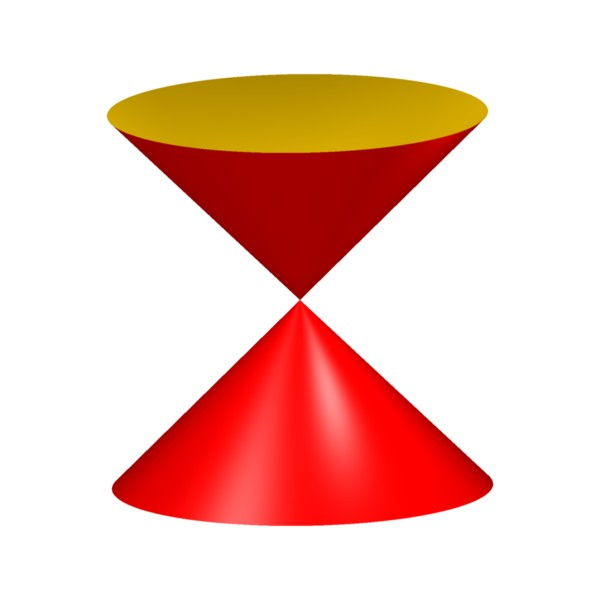
\includegraphics[width=1.2cm]{./../../common/images/A1pm_1} 
        \end{tabular}
        &
        $\rightarrow$
        &
        \begin{tabular}{@{}c@{}}
          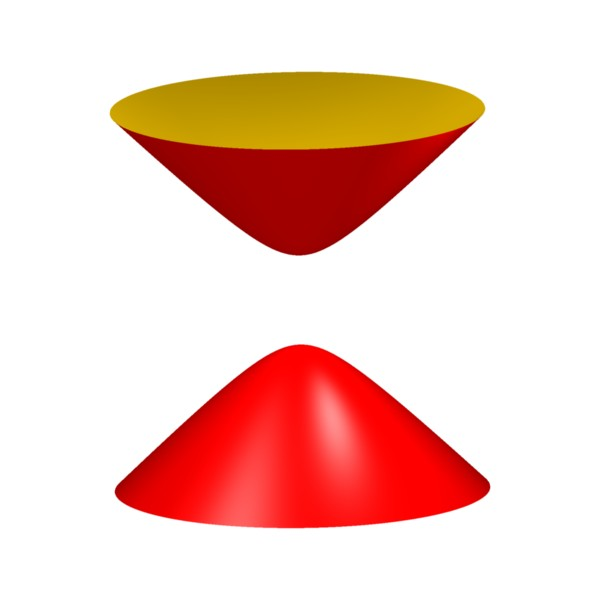
\includegraphics[width=1.2cm]{./../../common/images/A1pm_0}
        \end{tabular}
      \end{tabular}
    \end{center}
%    }
    \vspace{-0.2cm}
   $2$차 곡면은 $1$개 이상의 특이점을 가질 수 없습니다. 그러므로 $\mu(2)=1$ 이라고 할 수 있겟죠!
\end{surferPage}
